\documentclass[11pt, twoside, pdftex]{article}

% This include all the settings that we should use for the document
\newcommand{\PDFTitle}{Using HAL Device Drivers with the \productNameMed{}}
\newcommand{\commonPath}{../../Common}
\newcommand{\datePublished}{Mar 2022}

\newcommand{\versnum}{21.1} %version number quartus/AMP
\newcommand{\quartusname}{Quartus\textsuperscript{\textregistered} Prime}	
\newcommand{\textBar}{For \quartusname{} \versnum{}}
\newcommand{\thisyear}{2022 } %for copyright
\newcommand{\company}{FPGAcademy.org}
\newcommand{\longteamname}{FPGAcademy.org}
\newcommand{\teamname}{FPGAcademy}
\newcommand{\website}{FPGAcademy.org}

\newcommand{\productAcronym}{AMP}
\newcommand{\productNameShort}{Monitor Program}

\newcommand{\productNameMedTM}{Monitor Program}
\newcommand{\productNameMed}{Monitor Program}

%\newcommand{\headerLogoFilePath}[1]{#1/FPGAcademy.png}



\setlength\topmargin{-0.25in}
\setlength\headheight{0in}
\setlength\headsep{0.35in}
\setlength\textheight{8.5in}
\setlength\textwidth{7in}
\setlength\oddsidemargin{-0.25in}
\setlength\evensidemargin{-0.25in}
\setlength\parindent{0.25in}
\setlength\parskip{0in} 

\pdfpagewidth 8.5in
\pdfpageheight 11in

% listings is a package that supports encapsulating source code in LaTeX conveniently

\usepackage{listings}
% add support for graphics
\usepackage{graphicx}
\usepackage[usenames, dvipsnames]{color}

\def\expandparam\lstinputlisting[#1]#2{\edef\tmp{\noexpand\lstinputlisting[#1]{#2}}\tmp}

\widowpenalty 10000
\clubpenalty 10000

%%%%%%%%%%%%%%%%%%%% Source Code Formatting %%%%%%%%%%%%%%%%%%%%
\definecolor{globalCommentColour}{rgb}{0.588,0.588,0.588}

%%%%%%%%%%%%%%%%%%%%%%%%%%%%%%%%%%%%%%%%%%%%%%%%%%%%
% Defining a NiosII ASM highlighter for lstlisting
\lstdefinelanguage[NiosII]{Assembler} {
 	morekeywords={add, addi, and, andhi, andi, beq, bge, bgeu, bgt, bgtu, ble,  bleu, blt, bltu, bne, br, break,% 
 	bret, call, callr, cmpeq, cmpeqi, cmpge, cmpgei, cmpgeu, cmpgeui, cmpgt, cmpgti, cmpgtu, cmpgtui, cmple,%
 	cmplei, cmpleu, cmpleui, cmplt, cmplti, cmpltu, cmpltui, cmpne, cmpnei, custom, div, divu, eret, flushd,%
 	flushda, flushi, flushp, initd, initda, initi, jmp, jmpi, ldb, ldbio, ldbu, ldbuio, ldh, ldhio, ldhu, ldhuio,%
 	ldw, ldwio, mov, movhi, movi, movia, movui, mul, muli, mulxss, mulxsu, mulxuu, nextpc, nop, nor, or, orhi, ori,%
 	rdctl, rdprs, ret, rol, roli, ror, sll, slli, sra, srai, srl, srli, stb, stbio, sth, sthio, stw, stwio,%
 	sub, subi, sync, trap, wrctl, wrtcl, wrprs, xor, xori, xorhi, xori},% 	
 	morekeywords=[2]{.abort, .ABORT, .align, .app-file, .ascii, .asciz, .balign, .byte, .comm, .data, .def,%
 	.desc, .dim, .double, .eject, .else, .end, .endef, .endif, .equ, .equiv, .err, .extern, .file, .fill, .float,%
 	.global, .globl, .hword, .ident, .if, .include, .int, .irp, .irpc, .lcomm, .lflags, .line, .linkonce, .ln,%
 	.list, .long, .macro, .mri, .nolist, .octa, .org, .p2align, .psize, .quad, .rept, .sbttl, .scl, .section,%
 	.set, .short, .single, .size, .sleb128, .skip, .space, .stadb, .stabn, .stabs, .string, .symver, .tag,%
 	.text, .title, .type, .val, .uleb128, .word},% 	
 	morekeywords=[3]{et, bt, gp, sp, fp, ea, sstatus, ra, pc, status, estatus, bstatus, ienable, ipending, cpuid,%
 	exception, pteaddr, tlbacc, tlbmisc, eccinj, badaddr, config, mpubase, mpuacc},% 	
 	sensitive=t,%
 	alsoletter=.,%
	morestring=[b]",%
 	morecomment=[s]{/*}{*/},%
 	morecomment=[l]\#,%
   }[keywords,comments,strings]
   
   %% NOTE: morekeywords=[2] are GNU directives.
   
   \definecolor{niosInstructionColour}{rgb}{0.000,0.608,0.000}
   \definecolor{niosDirectiveColour}{rgb}{0.000,0.000,0.902}
   \definecolor{niosSpecialRegColour}{rgb}{0.000,0.000,0.000}
   \definecolor{niosStringColour}{rgb}{0.808,0.482,0.000}
   
   %% NOTE: To make bold use: =\bfseries\color{<colour>}
   \lstdefinestyle{defaultNiosStyle} {
   language=[NiosII]{Assembler},
   stringstyle=\color{niosStringColour},
   keywordstyle=\color{niosInstructionColour},
   keywordstyle=[2]\color{niosDirectiveColour},
   keywordstyle=[3]\itshape\color{niosSpecialRegColour}
   }
%%%%%%%%%%%%%%%%%%%%%%%%%%%%%%%%%%%%%%%%%%%%%%%%%%%%

%%%%%%%%%%%%%%%%%%%%%%%%%%%%%%%%%%%%%%%%%%%%%%%%%%%%
% Defining a ArmA9 ASM highlighter for lstlisting
\lstdefinelanguage[ArmA9]{Assembler} {
 	morekeywords={ADC, ADD, ADDS, AND, ANDS, B, BAL, BEQ, BGE, BGT, BL, BLT, BIC, BKPT, BLX, BNE, BX, CDP, CLZ, CMN, CMP, EOR,%
 	EORS, LDC, LDM, LDR, LDRB, LDRBT, LDRH, LDRSB, LDRSH, LDRT, LSL, MCR, MLA, MOV, MOVW, MOVT, MRC, MRS, MSR, MUL, MVN, ORR, PLD,%
 	ROR, RSB, RSC, SBC, SMLAL, SMULL, STC, STM, STR, STRB, STRBT, STRH, STRT, SUB, SUBS, SWI, SWP, SWPB, TEQ, UMLAL,
 	PUSH, POP, MOVS, RORS, LSR},%
 	morekeywords=[2]{.abort, .ABORT, .align, .app-file, .ascii, .asciz, .balign, .byte, .comm, .data, .def,%
 	.desc, .dim, .double, .eject, .else, .end, .endef, .endif, .equ, .equiv, .err, .extern, .file, .fill, .float,%
 	.global, .globl, .hword, .ident, .if, .include, .int, .irp, .irpc, .lcomm, .lflags, .line, .linkonce, .ln,%
 	.list, .long, .macro, .mri, .nolist, .octa, .org, .p2align, .psize, .quad, .rept, .sbttl, .scl, .section,%
 	.set, .short, .single, .size, .sleb128, .skip, .space, .stadb, .stabn, .stabs, .string, .symver, .tag,%
 	.text, .title, .type, .val, .vectors, .uleb128, .word},%
 	morekeywords=[3]{SP, PC, MIDR, CTR, TCMTR, TLBTR, MPIDR, ID_PFR0, ID_PFR1, ID_DFR0, ID_MMFR0, ID_MMFR1, ID_MMFR2,%
 	ID_MMFR3, ID_ISAR0, ID_ISAR1, ID_ISAR2, ID_ISAR3, ID_ISAR4, CCSIDR, CLIDR, AIDR, CSSELR, TTBR0, TTRB1, TTBR2, DACR,%
 	DFSR, IFSR, ADFSR, AIFSR, DFAAR, IFAR, ICIALLUIS, BPIALLIS, PAR, ICIALLU, ICIMVAU, BPIALL, DCIMVAC, DCISW, V2PCWPR,%
 	DCCVAC, DCCSW, DDIMVAC, DCISW, TLBALLIS, TLBIMVAIS, TLBIASIDIS, TLBIMVAAIS, TLBIALL, TLBIMVA, TLBIASID, TLBIMVAA,%
 	PMCR, PMCNTENSET, PMCNTENCLR, PMOVSR, PMSWINC, PMSELR, PMXEVTYPER, PMXEVCNTR, PMUSERENR, PMINTENSET, PMINTENCLR,%
 	PRRR, NRRR, PLEIDR, PLEASR, PLEFSR, PLEUAR, PLEPCR, VBAR, MVBAR, ISR, FCSEIDR, CONTEXTIDR, TPIDRURW, TPIDRURO, TPIDRPRW},%
 	sensitive=f,%
 	alsoletter=.,%
	morestring=[b]",%
 	morecomment=[s]{/*}{*/},%
 	morecomment=[l]{//},%
   }[keywords,comments,strings]
   
   %% NOTE: morekeywords=[2] are GNU directives.
   
   \definecolor{armInstructionColour}{rgb}{0.000,0.608,0.000}
   \definecolor{armDirectiveColour}{rgb}{0.000,0.000,0.902}
   \definecolor{armSpecialRegColour}{rgb}{0.000,0.000,0.000}
   \definecolor{armStringColour}{rgb}{0.808,0.482,0.000}
   
   \lstdefinestyle{defaultArmStyle} {
   language=[ArmA9]{Assembler},
   stringstyle=\color{armStringColour},
   keywordstyle=\color{armInstructionColour},
   keywordstyle=[2]\color{armDirectiveColour},
   keywordstyle=[3]\itshape\color{armSpecialRegColour}
   }
%%%%%%%%%%%%%%%%%%%%%%%%%%%%%%%%%%%%%%%%%%%%%%%%%%%%

%%%%%%%%%%%%%%%%%%%%%%%%%%%%%%%%%%%%%%%%%%%%%%%%%%%%
% Defining style for the verilog.

\definecolor{verilogCommentColour}{rgb}{0.000,0.502,0.000}

\lstdefinestyle{defaultVerilogStyle} {
language={Verilog},
keywordstyle=\color{blue},
commentstyle=\color{verilogCommentColour}
}
%%%%%%%%%%%%%%%%%%%%%%%%%%%%%%%%%%%%%%%%%%%%%%%%%%%%

%%%%%%%%%%%%%%%%%%%%%%%%%%%%%%%%%%%%%%%%%%%%%%%%%%%%
% Defining style for the vhdl.
\lstdefinestyle{defaultVHDLStyle} {
language={VHDL},
keywordstyle=\color{blue},
commentstyle=\color{verilogCommentColour}
}
%%%%%%%%%%%%%%%%%%%%%%%%%%%%%%%%%%%%%%%%%%%%%%%%%%%%

%%%%%%%%%%%%%%%%%%%%%%%%%%%%%%%%%%%%%%%%%%%%%%%%%%%%
% Java
\definecolor{javaStringColour}{rgb}{0.808,0.482,0}
%%%%%%%%%%%%%%%%%%%%%%%%%%%%%%%%%%%%%%%%%%%%%%%%%%%%

%%%%%%%%%%%%%%%%%%%%%%%%%%%%%%%%%%%%%%%%%%%%%%%%%%%%
% Defining language styles
% C
\definecolor{CStringColour}{rgb}{0.808,0.482,0}
%%%%%%%%%%%%%%%%%%%%%%%%%%%%%%%%%%%%%%%%%%%%%%%%%%%%

%%%%%%%%%%%%%%%%%%%%%%%%%%%%%%%%%%%%%%%%%%%%%%%%%%%%
% Defining extended LaTeX language.
\lstdefinelanguage[LocalLaTeX]{TeX}[LaTeX]{TeX}%
 	{moretexcs={bf, it, sf, lstset},%
   	}%

\lstdefinestyle{defaultLocalLatexStyle} {
language=[LocalLatex]{TeX},
keywordstyle=\color{blue}\bfseries,
keywordstyle=[2]\color{blue},
keywordstyle=[3]\color{blue}\bfseries
}
%%%%%%%%%%%%%%%%%%%%%%%%%%%%%%%%%%%%%%%%%%%%%%%%%%%%

\lstset{
%language = C,
%language = Verilog,
%basicstyle=\color{black}\rmfamily\ttfamily,
basicstyle=\small\color{black}\ttfamily,
commentstyle=\small\color{globalCommentColour}\itshape\ttfamily,
keywordstyle=\small\color{blue}\bfseries\ttfamily,
showstringspaces=false,
frame=none, %lines % boxed listings
breaklines=true,
breakatwhitespace=true,
tabsize=4
}
%%%%%%%%%%%%%%%%%%%%%%%%%%%%%%%%%%%%%%%%%%%%%%%%%%%%%%%%%%%%%%%%


%\usepackage[centering]{geometry}.
%%%%%%%%%%%%%%%%%%%%%%%%%%%%%%%%%%%%%%%%%%%%%%%%%%%
% Document Settings
\usepackage[labelsep=period]{caption}
% we can choose a better font later
%\usepackage{palatino}
\usepackage{fourier}
%\fontencoding{T1}
% include common used symbols
\usepackage{textcomp}
% add support for graphics
\usepackage{graphicx}
\usepackage[usenames, dvipsnames]{color}
% enable to draw thick or thin table hlines
\setlength{\doublerulesep}{\arrayrulewidth}
\usepackage{longtable}
\setlongtables
%\usepackage{array}
% It may be better to use PDFLaTeX as it can generate bookmarks for the
% document

% Add some useful packages
\usepackage{ae,aecompl}
\usepackage{epsfig,float,times}

% reset the font for section
\usepackage{sectsty}
%\allsectionsfont{\fontfamily{ptm}\selectfont}
\allsectionsfont{\usefont{OT1}{phv}{bc}{n}\selectfont}

% use compact space for sections
\usepackage[compact]{titlesec}
\titlespacing{\section}{0pt}{0.2in}{*0}
\titlespacing{\subsection}{0pt}{0.1in}{*0}
\titlespacing{\subsubsection}{0pt}{0.05in}{*0}

% fancyhdr header and footer customization
\usepackage{layout}
\usepackage{fancyhdr}
\pagestyle{fancy}
\fancyhead{}
\fancyhead[R]{\textit{\tiny{\textBar}}}
\fancyfoot{}
\fancyfoot[LO,
RE]{\textrm{\href{https://www.fpgacademy.org}{\small \longteamname}} \\ {\small \datePublished }}
\fancyfoot[RO, LE]{\small \thepage}
% two-side settings
%\fancyhead{} % clear all header fields
%\fancyfoot{} % clear all footer fields
%\fancyfoot[LE,RO]{\thepage}
\renewcommand{\headrulewidth}{2pt}
\renewcommand{\headrule}{{\color{blue} \hrule width\headwidth height\headrulewidth \vskip-\headrulewidth}}
\renewcommand{\footrulewidth}{0pt}

% Format the footer on page 1
\fancypagestyle{plain}{
\fancyhead{}
\fancyfoot{}
\fancyfoot[LO,
RE]{\textrm{\href{https://www.fpgacademy.org}{\small \longteamname}} \\ {\small \datePublished }}
\fancyfoot[RO, LE]{\small \thepage}
\renewcommand{\headrulewidth}{0pt}
}
% adjust some setting to try to make the figure stay in the same page with text
% Reference: 	http://www.cs.uu.nl/~piet/floats/node1.html
%   			http://mintaka.sdsu.edu/GF/bibliog/latex/floats.html
%   General parameters, for ALL pages:
\renewcommand{\topfraction}{0.9}	% max fraction of floats at top
\renewcommand{\bottomfraction}{0.8}	% max fraction of floats at bottom
%   Parameters for TEXT pages (not float pages):
\setcounter{topnumber}{3}
\setcounter{bottomnumber}{3}
\setcounter{totalnumber}{5}     % 2 may work better
\setcounter{dbltopnumber}{2}    % for 2-column pages
\renewcommand{\dbltopfraction}{0.9}	% fit big float above 2-col. text
\renewcommand{\textfraction}{0.07}	% allow minimal text w. figs
%   Parameters for FLOAT pages (not text pages):
\renewcommand{\floatpagefraction}{0.7}	% require fuller float pages
% N.B.: floatpagefraction MUST be less than topfraction !!
\renewcommand{\dblfloatpagefraction}{0.7}	% require fuller float pages
%%%%%%%%%%%%%%%%%%%%%%%%%%%%%%%%%%%%%%%%%%%%%%%%%%%
% remember to use [htp] or [htpb] for placement
%%%%%%%%%%%%%%%%%%%%%%%%%%%%%%%%%%%%%%%%%%%%%%%%%%%

% set no indent for paragraph
\setlength{\parindent}{0em}
\addtolength{\parskip}{11pt}
\newcommand{\compact}{[topsep=0pt]}
% use this package to reduce space
\usepackage{enumitem}
\usepackage{multirow}
\usepackage{rotating}
\usepackage{pifont}
\usepackage{dingbat}
\newcommand{\itemsecond}{$\circ$}
%
%%%%%%%%%%%%%%%%%%
\date{}
\author{}
%%%%%%%%%%%%%%%%%%
\newcommand{\de}{DE-series}
\newcommand{\up}{FPGAcademy}
\newcommand{\fabric}{Avalon Switch Fabric}
\newcommand{\TODO}[1]{\textcolor{red}{\textbf{TODO}: #1}}
\def\registered{{\ooalign{\hfil\raise .00ex\hbox{\scriptsize R}\hfil\crcr\mathhexbox20D}}}

% enable url and reference(bookmarks) in pdf
\usepackage{url}
\usepackage[pdftex, colorlinks]{hyperref}
\hypersetup{%
pdftitle={\PDFTitle},
linkcolor=blue,
hyperindex=true,
pdfauthor={\longteamname},
pdfkeywords={FPGAcademy, Academic Program, Example System},
bookmarksnumbered,
bookmarksopen=false,
filecolor=blue,
pdfstartview={FitH},
urlcolor=blue,
plainpages=false,
pdfpagelabels=true,
linkbordercolor={1 1 1} %no color for link border
}%
%%%%%%%%%%%%%%%%%%%%%%%%%%%%%%%%%%%%%%%%%%%%%%%%%%%
\setlength{\fboxsep}{0.7pt}
\setlength{\fboxrule}{0.5pt}

\newcommand{\red}[1]{{\color{red}\sf{#1}}}
\newcommand{\blue}[1]{{\color{blue}\sf{#1}}}



%%%%%%%%%%%%%%%%%%%%%%%%%
% Add title
\newcommand{\doctitle}{Using HAL Device Drivers \\ with the \productNameMed{}}
\newcommand{\dochead}{Using HAL Device Drivers with the \productNameMed{}}
% Usually no need to change these two lines
\title{\fontfamily{phv}\selectfont{\doctitle} }
\chead{ \small{\textsc{\bfseries \dochead} } }
% Customizations
%%%%%%%%%%%%%%%%%%%%%%%%%

%%%%%%%%%%%%%%%%%%
%%% DOCUMENT START
%\begin{document}
\begin{document}
\begin{table}
    \centering
    \begin{tabular}{p{5cm}p{4cm}}
        \hspace{-3cm}
        &
        \raisebox{1\height}{\parbox[h]{0.5\textwidth}{\Large\fontfamily{phv}\selectfont{\textsf{\doctitle}}}}
    \end{tabular}
    \label{tab:logo}
\end{table}

\colorbox[rgb]{0,0.384,0.816}{\parbox[h]{\textwidth}{\color{white}\textsf{\textit{\textBar}}}}

\thispagestyle{plain}
 
\section{Introduction}

This tutorial shows how to develop C programs that use device driver functions for the I/O devices in a
Nios\textsuperscript{\textregistered} II hardware system. The device driver functions used in the tutorial are provided as part of the Intel\textsuperscript{\textregistered} FPGA University
Program IP cores, which are available from the University Program section of Intel's website. These 
functions are implemented using Intel's Hardware Abstraction Layer (HAL). In addition to 
providing support for device drivers, the HAL simplifies many programming tasks, such as the development of 
programs that use interrupts. A detailed description of the features provided by the HAL can be found in the
{\it Nios~II Software Developer's Handbook}, which is available from Intel.

The Nios~II software programs shown in the tutorial are implemented by using 
the \productNameMed{} development environment.
This tutorial includes screen captures obtained using version \versnum of the
\productNameMed{}; if other versions of the software are used, some of the
images may be slightly different. The device driver functions used in the example programs in the tutorial are from version \versnum~ of the University Program IP Cores.

We assume that the reader has access to the Intel DE2-115 Development 
and Education board, or the DE1-SoC board. If other boards are used, then the design examples
for the tutorial may be not usable, as they require the presence of specific I/O devices.
 
 
{\bf Contents}:
\begin{itemize}
\item Examining the HAL device driver functions that are provided for University Program IP cores
\item Writing C programs that use HAL device driver functions
\item Compiling HAL code with the Monitor Program
\item Running and debugging HAL code using the Monitor Program
\item Finding HAL device driver source code
\item Using Nios~II interrupts in HAL code
\end{itemize}
\clearpage
\newpage
\section{Writing Programs that use HAL Device Drivers}

For this tutorial, we assume that the reader is already familiar with the \productNameMed{}. It is
described in the tutorial {\it Introduction to 
the \productNameMed{}}, which is available from the FPGA University Program section of Intel's website.

To see an example of using HAL device drivers, create a new Monitor Program project for the 
DE2-115 board called {\it HAL\_tutorial}. Store the project in a directory of your choice. 
When creating the project, specify the hardware system to be the prebuilt {\it DE2-115 Computer System},
specify the program type as {\sf Program with Device Driver Support}, check {\sf Include a sample program with the project},
 and select the sample program named {\it Audio}.  This sample program makes use of two types of I/O devices 
in the DE2-115 Computer System: parallel ports, and an audio device.

The HAL device drivers for I/O devices consist of collections of functions that allow software
programs to access hardware devices. To use these functions, it is first necessary 
to examine the documentation provided for the IP core that connects to each I/O device, to 
determine the names of its device driver functions, the number 
and types of arguments, and the specified use of the functions. The documentation
for the IP cores that are included in the DE2-115 Computer System can be found on the University 
Program section of Intel's website under the heading {\sf Materials > Computer 
Organization > IP Cores}. As an example, the documentation file for the 
parallel ports provides a section called {\it Programming with the Parallel Ports}.  A small part of 
this section is displayed in Figure~\ref{fig:parallel_port_doc}.  
A number of device driver functions are listed in the figure,
including {\it alt\_up\_parallel\_port\_open\_dev($\ldots$)}, which is used in C code to open 
a parallel port device, as well as {\it alt\_up\_parallel\_port\_read\_data($\ldots$)} and
{\it alt\_up\_parallel\_port\_write\_data($\ldots$)}, which can be used to read/write data from/to 
a parallel port. For each function, the documentation specifies the data types 
of arguments and return values.

\clearpage
\begin{figure}[h!]
   \begin{center}
      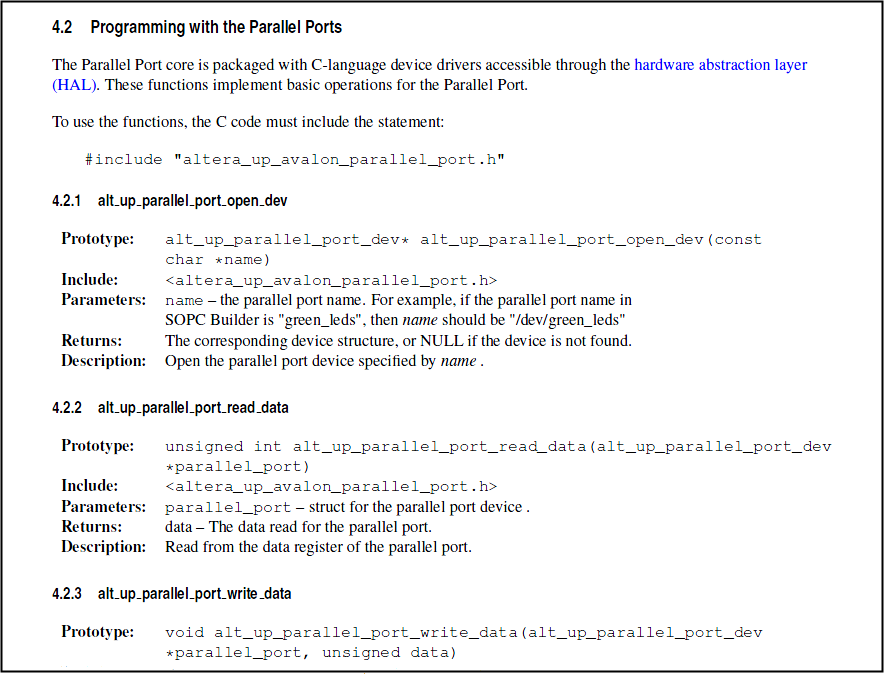
\includegraphics[scale=0.65]{figures/parallel_port_doc.png}
   \end{center}
   \caption{A part of the documentation file for the parallel port.} 
	\label{fig:parallel_port_doc}
\end{figure}

The sample program {\it Audio} is given as a complete example of C code that uses HAL device drivers.
The C code is shown in Figure~\ref{fig:HAL_audio}. This code uses two parallel ports, connected to
switches and LEDs on the DE2-115 board, and an audio port. The code performs the following operations:
\begin{enumerate}
\item When the switch {\it KEY}$_1$ is pressed on the DE2-115 board, audio input from the microphone jack is recorded for 
about 10 seconds. {\it LEDG}$_0$ is illuminated while recording.
\item When the switch {\it KEY}$_2$ is pressed, the recorded audio is played back on the line-out jack. {\it LEDG}$_1$
is illuminated during playback.
\end{enumerate}

\noindent
As shown in Figure~\ref{fig:HAL_audio}($a$), the C code first includes the necessary header files for the parallel
port and audio devices. In lines $7 - 9$ a pointer is declared for each of the three I/O devices to be used in
the code. The pointers have a special type, which is the type of return value for the device driver function that opens
the device--for example, in Figure~\ref{fig:parallel_port_doc} the data type of the 
function {\it alt\_up\_parallel\_port\_open\_dev($\ldots$)} is {\it alt\_up\_parallel\_port\_dev}. Lines $10-12$
of the code open the two parallel ports and the audio device needed in the program. As shown, each I/O
device is referenced using a unique name. The names of the two parallel port devices are {\it Pushbuttons} and 
{\it Green\_LEDs}, and the audio device is named {\it Audio\_Subsystem\_Audio}. These names are prefixed with the string
{\it /dev/}, and then passed to the device driver function. The unique name of each device is assigned by the
designer when the Nios~II hardware system is created by using Intel's Platform Designer tool.
Figure~\ref{fig:Qsys_DE2_Media} shows part of the {\it Systems Contents} that can be displayed in the Platform Designer 
tool for the DE2-115 Computer System, with the module names (without the {\it /dev/ prefix}) displayed in the column 
labeled {\it Module Name}. Figure~\ref{fig:Qsys_Audio_Subsystem} shows the {\it Systems Contents} that can be displayed in the Platform Designer 
tool for the Audio Subsystem, with the module names (without the {\it /dev/Audio\_Subsystem\_ prefix}) displayed in the column labeled {\it Module Name}.

\begin{figure}[h!]
\begin{center}
\begin{minipage}[t]{12.5 cm}
\begin{tabbing}
000 \=\#{\bf define} BUF\_SIZE 500000ZZZZZZ\=// about 10 seconds of buffer (@ 48K samples/sec)\kill
1 \>\#{\bf include} "altera\_up\_avalon\_parallel\_port.h"\\
2 \>\#{\bf include} "altera\_up\_avalon\_audio.h"\\
 
\>/* globals */\\
3 \>\#{\bf define} BUF\_SIZE 500000	\>// about 10 seconds of buffer (@ 48K samples/sec)\\
4 \>\#{\bf define} BUF\_THRESHOLD 96	\>// 75\% of 128 word buffer \\
 
\>/* function prototypes */\\
5 \>{\bf void} check\_KEYs( {\bf int} *, {\bf int} *, {\bf int} *, alt\_up\_parallel\_port\_dev *, alt\_up\_audio\_dev * );\\
000 \=/\=*****\=***\=******************************\=****************************************\=\kill
\rule{6.0in}{0in} 
\>/********************************************************************************\\
\>\>* This program demonstrates use of the media ports in the DE2-115 Computer System\\
\>\>*\\
\>\>* It performs the following: \\
\>\>*  	\>1. \>records audio for about 10 seconds when KEY[1] is pressed. LEDG[0] is\\
\>\>*  	\>\>   lit while recording\\
\>\>* 	\>2. \>plays the recorded audio when KEY[2] is pressed. LEDG[1] is lit while \\
\>\>* 	\>\>   playing\\
000 \=\=\kill\\
\>\>********************************************************************************/\\
000 \=ZZZ\=ZZZ\={\bf define} BUF\_SIZE 500000ZZZZZZ\=// about 10 seconds of buffer \kill
6 \>{\bf int} main({\bf void})\\
\>\{\\
\>\>/* declare variables to point to devices that are opened */\\
7	\>\>alt\_up\_parallel\_port\_dev *KEY\_dev;\\
8	\>\>alt\_up\_parallel\_port\_dev *green\_LEDs\_dev;\\
9	\>\>alt\_up\_audio\_dev *audio\_dev;\\
 
\>\>// open the pushbutton KEY parallel port\\
10\>\>KEY\_dev = alt\_up\_parallel\_port\_open\_dev ("/dev/Pushbuttons");\\
\>\>// open the green LEDs parallel port\\
11\>\>green\_LEDs\_dev = alt\_up\_parallel\_port\_open\_dev ("/dev/Green\_LEDs");\\
\>\>// open the audio port\\
12\>\>audio\_dev = alt\_up\_audio\_open\_dev ("/dev/Audio\_Subsystem\_Audio");\\
 
\>\>/* used for audio record/playback */\\
13\>\>{\bf int} record = 0, play = 0, buffer\_index = 0;\\
14\>\>{\bf unsigned int} l\_buf[BUF\_SIZE];\\
15\>\>{\bf unsigned int} r\_buf[BUF\_SIZE];\\
16\>\>{\bf int} num\_read; int num\_written;\\
\end{tabbing}
\end{minipage}
\end{center}
	\vspace{-0.33in}\caption{An example of C code that uses HAL device drivers (Part $a$).}
   \label{fig:HAL_audio}
\end{figure}
\clearpage

The rest of the code in Figure~\ref{fig:HAL_audio} performs the recording and playback of audio, and controls
the pushbutton and green lights parallel ports. Device driver functions are called in the main program in 
lines $22$, 24$-$25, 29, 31, 33$-$34, and 38, and in the function {\it check\_KEYs}, which examines
the values of the pushbutton switches, in lines 41$-$42, 45, and 49. The operation of each of these functions is 
described in the documentation file for the corresponding IP core, as discussed previously for 
Figure~\ref{fig:parallel_port_doc}.

\begin{table}
\begin{center}
\begin{minipage}[t]{12.5 cm}
\begin{tabbing}
000 \=ZZZ\=ZZZ\=ZZZ\=ZZZ\=ZZZ\=ZZZ\={\bf define} BUF\_SIZE 500000ZZZZZZ\=// about 10 seconds \kill
\rule{6.0in}{0in} 
\>\>/* read and echo audio data */\\
17\>\>record = 0;\\
18\>\>play = 0;\\
19\>\>{\bf while}(1)\\
\>\>\{\\
20\>\>\>check\_KEYs (\&record, \&play, \&buffer\_index, KEY\_dev, audio\_dev);\\
21\>\>\>{\bf if} (record)\\
\>\>\>\{\\
22\>\>\>\>alt\_up\_parallel\_port\_write\_data (green\_LEDs\_dev, 0x1); ~~// set LEDG[0] on\\
 
\>\>\>\>// record data until the buffer is full\\
23\>\>\>\>{\bf if} (buffer\_index < BUF\_SIZE)\\
\>\>\>\>\{\\
24\>\>\>\>\>num\_read = alt\_up\_audio\_record\_r (audio\_dev, \&(r\_buf[buffer\_index]), \\
\>\>\>\>\>\>BUF\_SIZE - buffer\_index);\\
\>\>\>\>\>/* assume we can read same \# words from the left and right */\\
25\>\>\>\>\>({\bf void}) alt\_up\_audio\_record\_l (audio\_dev, \&(l\_buf[buffer\_index]), num\_read);\\
26\>\>\>\>\>buffer\_index += num\_read;\\
 
27\>\>\>\>\>{\bf if} (buffer\_index =$\,$= BUF\_SIZE)\\
\>\>\>\>\>\{\\
\>\>\>\>\>\>// done recording\\
28\>\>\>\>\>\>record = 0;\\
29\>\>\>\>\>\>alt\_up\_parallel\_port\_write\_data (green\_LEDs\_dev, 0x0); ~~// turn off LEDG\\
\>\>\>\>\>\}\\
\>\>\>\>\}\\
\>\>\>\}\\
 
\>\>\>\>Figure~\ref{fig:HAL_audio}. An example of C code that uses HAL device drivers (Part $b$).
\end{tabbing}
\end{minipage}
\end{center}
\end{table}

\clearpage

\begin{table}
\begin{center}
\begin{minipage}[t]{12.5 cm}
\begin{tabbing}
000 \=ZZZ\=ZZZ\=ZZZ\=ZZZ\=ZZZ\=ZZZ\={\bf define} BUF\_SIZE 500000ZZZZZZ\=// about 10 seconds \kill
30\>\>\>{\bf else if} (play)\\
\>\>\>\{\\
31\>\>\>\>alt\_up\_parallel\_port\_write\_data(green\_LEDs\_dev, 0x2); ~~// set LEDG[1] on\\
\rule{6.0in}{0in} 
\>\>\>\>// output data until the buffer is empty \\
32\>\>\>\>{\bf if} (buffer\_index < BUF\_SIZE)\\
\>\>\>\>\{\\
33\>\>\>\>\>num\_written = alt\_up\_audio\_play\_r (audio\_dev, \&(r\_buf[buffer\_index]), \\
\>\>\>\>\>\>BUF\_SIZE - buffer\_index);\\
\>\>\>\>\>/* assume that we can write the same \# words to the left and right */\\
34\>\>\>\>\>({\bf void}) alt\_up\_audio\_play\_l (audio\_dev, \&(l\_buf[buffer\_index]), num\_written);\\
35\>\>\>\>\>buffer\_index += num\_written;\\
\\
36\>\>\>\>\>{\bf if} (buffer\_index =$\,$= BUF\_SIZE) ~~// done playback\\
\>\>\>\>\>\{\\
37\>\>\>\>\>\>play = 0;\\
38\>\>\>\>\>\>alt\_up\_parallel\_port\_write\_data(green\_LEDs\_dev, 0x0); ~~// turn off LEDG\\
\>\>\>\>\>\}\\
\>\>\>\>\}\\
\>\>\>\}\\
\>\>\}\\
\>\}\\
\\
\>/*********************************************************************************\\
\>\>* Subroutine to read KEYs\\
000 \=\=\kill
\>**********************************************************************************/\\
000 \={\bf void} check\_KEYs(\=int \kill
39\>{\bf void} check\_KEYs(int *KEY1, int *KEY2, int *counter, alt\_up\_parallel\_port\_dev *KEY\_dev,\\
\>\>alt\_up\_audio\_dev *audio\_dev)\\
000 \=ZZZ\=ZZZ\=ZZZ\=ZZZ\=ZZZ\=ZZZ\={\bf define} BUF\_SIZE 500000ZZZZZZZZZ\=// about 10 seconds \kill
\>\{\\
40\>\>{\bf int} KEY\_value;\\
41\>\>KEY\_value = alt\_up\_parallel\_port\_read\_data (KEY\_dev); \>\>\>\>\>\>// read the pushbutton KEY values\\
42\>\>{\bf while} (alt\_up\_parallel\_port\_read\_data (KEY\_dev)); \>\>\>\>\>\>// wait for pushbutton KEY release\\
43\>\>{\bf if} (KEY\_value =$\,$= 0x2)	\>\>\>\>\>\>// check KEY1\\
\>\>\{\\
44\>\>\>*counter = 0; \>\>\>\>\>// reset counter to start recording\\
45\>\>\>alt\_up\_audio\_reset\_audio\_core (audio\_dev); \>\>\>\>\>// reset audio port\\
46\>\>\>*KEY1 = 1;\\
\>\>\}\\
47\>\>{\bf else if} (KEY\_value =$\,$= 0x4) \>\>\>\>\>\>// check KEY2\\
\>\>\{\\
48\>\>\>*counter = 0; \>\>\>\>\>// reset counter to start playback\\
49\>\>\>alt\_up\_audio\_reset\_audio\_core (audio\_dev); \>\>\>\>\>// reset audio port\\
50\>\>\>*KEY2 = 1;\\
\>\>\}\\
\>\}\\
 
\>\>\>\>Figure~\ref{fig:HAL_audio}. An example of C code that uses HAL device drivers (Part $c$).
\end{tabbing}
\end{minipage}
\end{center}
\end{table}

\clearpage

\begin{figure}[h!]
   \begin{center}
      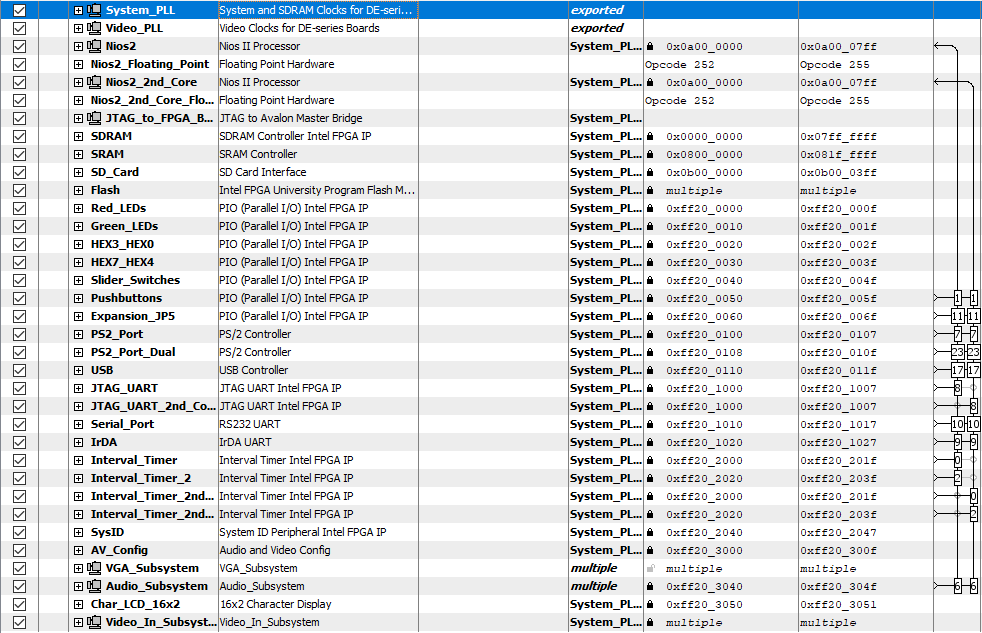
\includegraphics[scale=0.6]{figures/Qsys_DE2_Media.png}
   \end{center}
   \caption{Module names for the DE2-115 Computer System shown in Platform Designer.} 
	\label{fig:Qsys_DE2_Media}
\end{figure}

\begin{figure}[h!]
   \begin{center}
      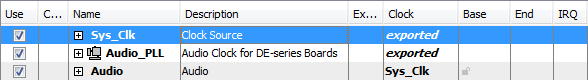
\includegraphics[scale=0.6]{figures/Qsys_Audio_Subsystem.png}
   \end{center}
   \caption{Module names for the DE2-115 Audio Subsystem shown in Platform Designer.} 
	\label{fig:Qsys_Audio_Subsystem}
\end{figure}

\section{Compiling Programs that use Device Drivers}
The {\it HAL\_tutorial} project can be compiled in the normal way by using the Monitor Program commands {\sf Actions >
Compile}, or {\sf Actions > Compile \& Load}. The first time this is done, the Monitor Program compiles not only the file 
{\it audio\_HAL.c}, but also a number of C library
functions that are a part of the HAL system, and all of the device driver functions that are provided 
for every device in the Nios~II hardware system. Although this process is somewhat time consuming, it is only done once, and 
subsequent compilations only compile the source file {\it audio\_HAL.c}. If it is necessary to recompile all of
the HAL functions at a later time, this can be accomplished by using the command {\sf Actions > Regenerate Device
Drivers (BSP)}. This action might be necessary, for example, if a new version of IP cores is installed at a later
time.

\subsection{Running the Program}

Programs that use HAL device drivers can be run and debugged in the Monitor Program in the same way as other C or 
assembly language programs. Figure \ref{fig:HAL_debug} shows an example of a breakpoint set in the code 
of Figure~\ref{fig:HAL_audio}. The figure shows
the value read from the pushbutton parallel port by the device driver function {\it
alt\_up\_parallel\_port\_read\_data}($\ldots$). This particular device driver is executed without using a {\it call}
assembly language instruction, which means that it is implemented as a macro, rather than a subroutine. The value 
returned by the function is shown in the Nios~II register {\it r3}. The value is \texttt{0x00000002}, which means 
that {\it KEY}$_1$ on the DE2-115 board was pressed when the function was called. Other device drivers are implemented as 
subroutines, such as {\it alt\_up\_audio\_record\_r}($\ldots$), as indicated in Figure~\ref{fig:HAL_debug_sub}. In
the figure, a breakpoint has been set at this function call. The subroutine can be executed in a debugging session 
by single-stepping into the device driver code if desired.
% either by using {\sf Actions > Step Over Subroutine} or by single-stepping into the device driver code if desired.

\begin{figure}[h!]
	\begin{center}
		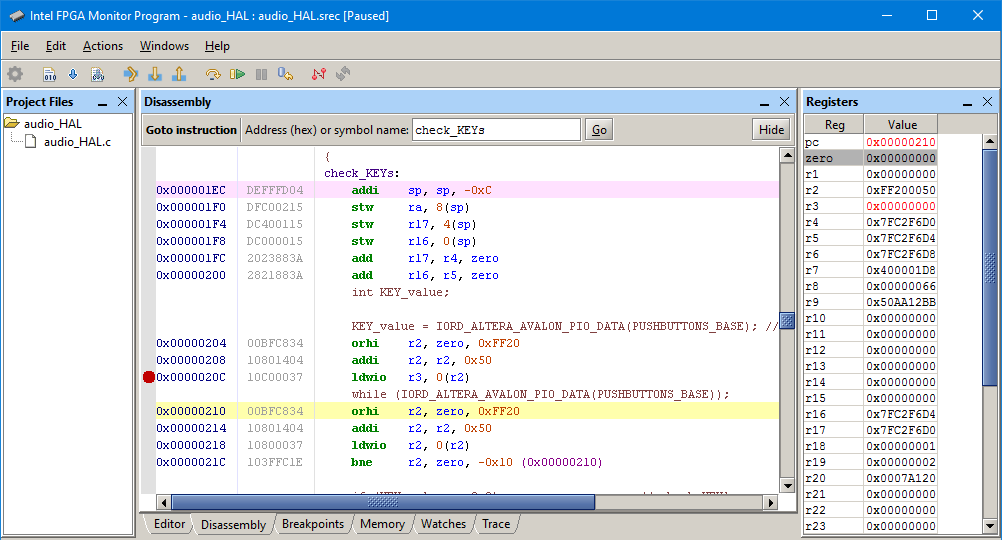
\includegraphics[width=5.75in]{figures/HAL_debug.png}
	\end{center}
	\caption{An example of a HAL device driver function that is implemented as a macro.} 
	\label{fig:HAL_debug}
\end{figure}

\begin{figure}[h!]
	\begin{center}
		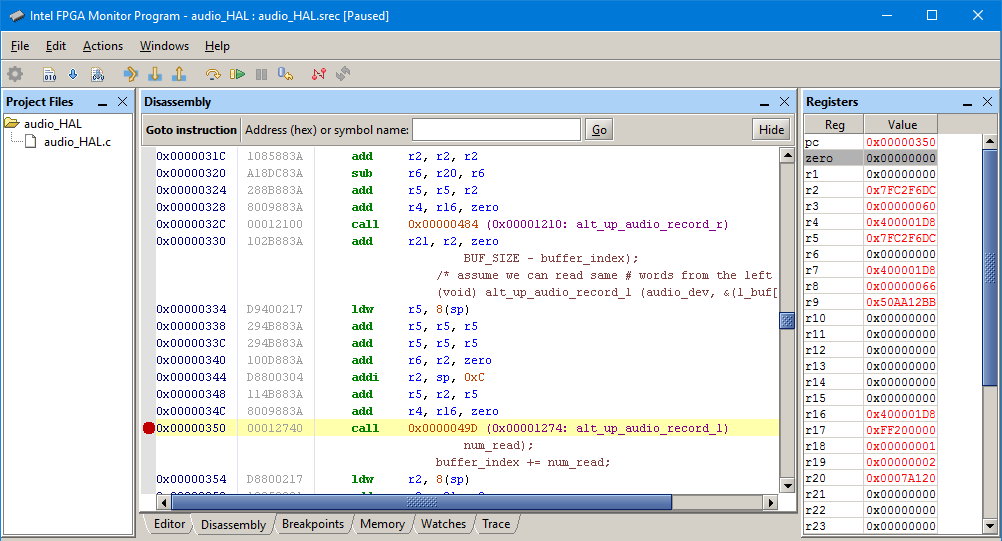
\includegraphics[width=5.75in]{figures/HAL_debug_sub.png}
	\end{center}
	\caption{An example of a HAL device driver function implemented as a subroutine.} 
	\label{fig:HAL_debug_sub}
\end{figure}

\section{Examining the HAL Device Driver Source Code}

It is possible to examine the source code of the device driver functions used in the HAL. These functions are installed
in the same filesystem directory as the Quartus\textsuperscript{\textregistered} Prime software, as illustrated on the left side of Figure~\ref{fig:folders}.
In this figure, \texttt{QUARTUS\_ROOTDIR} \footnote{In Windows operating systems, the environment variable 
\texttt{QUARTUS\_ROOTDIR} points to the folder where Quartus Prime software is installed.} represents the installation 
directory of the Quartus Prime software. The device driver code is stored in two directories: the {\it inc} directory contains 
device driver subroutine prototypes and device driver macros, and the {\it src} directory contains subroutine definitions. 
During the process of compiling a project in the Monitor Program, the {\it inc} and {\it src} directories for all IP cores
are copied into the project's directory. As shown on the right side of Figure~\ref{fig:folders}, the directories 
are copied into a folder called {\it drivers}, which is a subfolder of the folder called {\it BSP} (the acronym stands
for {\it Board Support Package}). The figure shows the directory structure of the parallel port and audio IP cores
as an example, but the source files for all of the IP cores in the hardware system are copied in this way.

\begin{figure}[h!]
   \begin{center}
      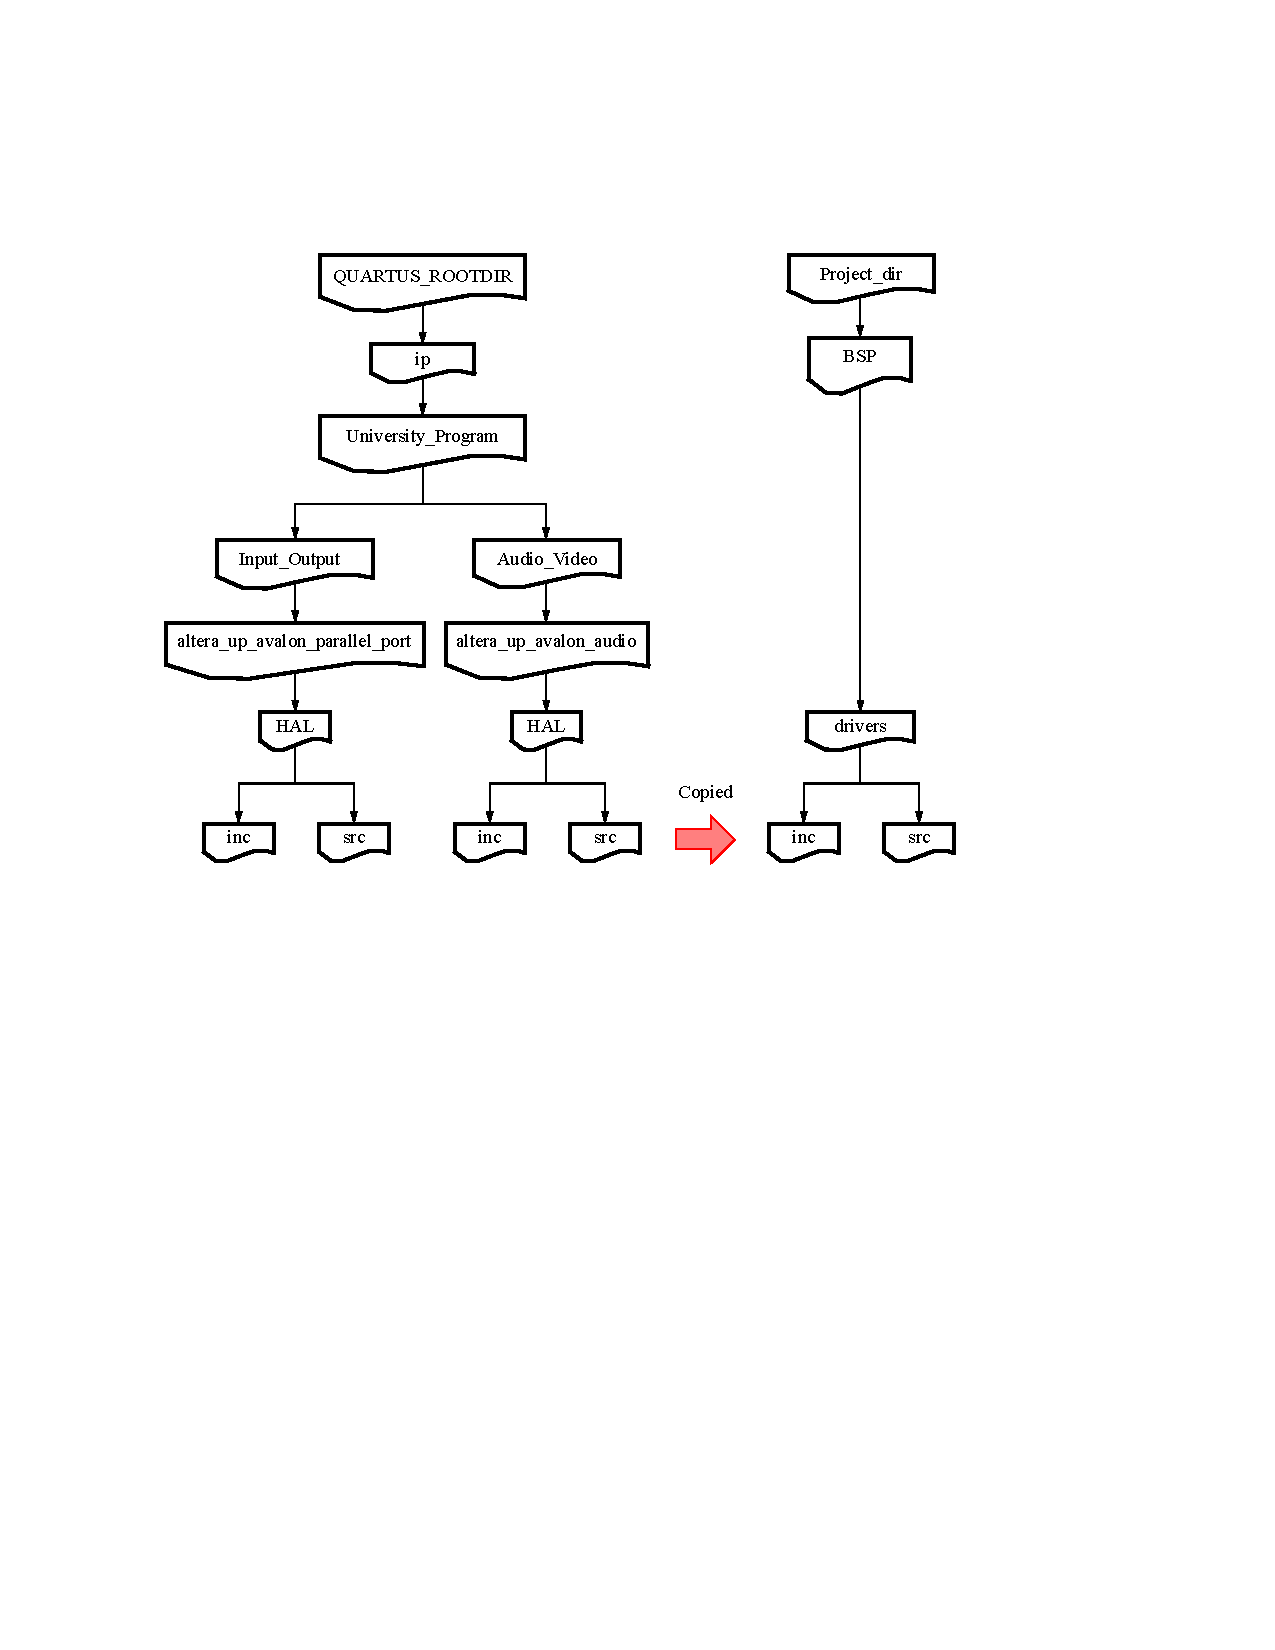
\includegraphics{figures/folders.pdf}
   \end{center}
   \caption{Finding the HAL device driver source code files.} 
	\label{fig:folders}
\end{figure}

\clearpage
\newpage
\section{Using Nios\textsuperscript{\textregistered} II Interrupts in the HAL}

The HAL provides a simple interface for using Nios~II interrupts in C programs. To use interrupts programs must 
specify the statement \#{\bf include} "sys/alt\_irq.h". This include file provides a function named 
{\it alt\_irq\_register ($\ldots$)}, which is used to specify the hardware interrupt levels and associated 
interrupt service routines for any Nios~II interrupts that are being used. To see an example that uses interrupts,
create a new Monitor Program project for the 
DE2-115 board called {\it HAL\_tutorial\_int}. Store the project in a directory of your choice. 
When creating the project, specify the hardware system to be the {\it DE2-115 Computer System},
specify the program type as {\sf Program with Device Driver Support}, check {\sf Include a sample program with the project}, 
and select the sample program provided in the Monitor Program named {\it interrupts\_example}.  This sample program has the exact same functionality 
as the code in
Figure~\ref{fig:HAL_audio}, except that the pushbutton {\it KEY} parallel port and audio device 
are handled using interrupts. There are three source files in this program:
{\it interrupts\_HAL.c} contains the main program, and the interrupt service routines are found in the files
{\it pushbutton\_ISR.c} and {\it audio\_ISR.c}.

Figure~\ref{fig:interrupts_HAL} shows the C code for the main program. It first includes the file {\it globals.h},
which, as illustrated in Figure~\ref{fig:globals_h}, includes the parallel port and audio HAL header files 
{\it altera\_up\_avalon\_parallel\_port.h} and {\it altera\_up\_avalon\_audio.h}.
The {\it globals.h} file also includes {\it sys/alt\_stdio.h} and
{\it alt\_irq.h}.  As mentioned above, {\it alt\_irq.h} is needed to use interrupts with the HAL. The file 
{\it alt\_stdio.h} defines some simplified versions of the functions in the standard C library {\it stdio.h}.
The purpose of {\it alt\_stdio.h} is to conserve memory space in the hardware system by providing functions that
have limited capability but also produce less machine code when compiled.  In this example, we will use a 
function called {\it alt\_printf}, which is a simplified version of {\it printf}. The use of such functions is
not necessary for the example program, and is provided only for illustrative purposes. The {\it alt\_stdio.h} 
library, and other C libraries provided by Intel, is described in the {\it Nios~II Software Developer's Handbook},
available from Intel's website.

The last few lines of code in Figure~\ref{fig:globals_h} declare a C structure named {\it alt\_up\_dev}. As indicated in
the code, this structure is used to hold a pointer to the I/O devices for the two parallel ports and audio port. We
will explain the purpose of this structure shortly. Referring back to the main program in
Figure~\ref{fig:interrupts_HAL}, line 2 defines an instance, named {\it up\_dev}, of the {\it alt\_up\_dev}
structure.  Line 3 defines two variables used with the audio device. 
These variables have to be declared using the keyword {\it
volatile}, because their values are written by interrupt service routines. If this keyword is not used, then the C
compiler may choose to save the value of the variable in a Nios~II general-purpose register and to retrieve the
value of this variable, when needed in a program, from this register, rather than from memory. In this case,
changes to the variable's value that are written into memory by an interrupt service routine would not be seen in 
the main program.  Using the {\it volatile} keyword prohibits the C compiler from saving the value of the variable 
in a CPU register, and causes the Nios~II processor to access the variable using 
{\it load I/O} and {\it store I/O} instructions \footnote{~Even if a version of the Nios~II 
processor that has a {\it data cache} is being used, the load
I/O instruction causes the processor to bypass this cache and access the associated variable at its address in memory.}.

\begin{figure}[h!]
\begin{center}
\begin{minipage}[t]{12.5 cm}
\begin{tabbing}
000 \=/\=* The globals below are written by interrupt service routines \kill
1\>\#{\bf include} "globals.h"\\
\>/* global variables */\\
000 \={\bf struct} alt\_up\_dev up\_dev;ZZZZZZZZZZZZZZZZZZ\=// holds a pointer to each \kill
2\>{\bf struct} alt\_up\_dev up\_dev;	\>// holds a pointer to each open I/O device\\
000 \=/\=* The globals below are written by interrupt service routines \kill
\>/* The globals below are written by interrupt service routines, so we have to declare \\
\>\>* them as volatile to avoid the compiler caching their values in registers */\\
000 \={\bf struct} alt\_up\_dev up\_dev;ZZZZZZZZZZZZZZZZZZ\=// holds a pointer to each \kill
3\>{\bf volatile int} buf\_index\_record, buf\_index\_play;	\>// audio variables\\
\>/* function prototypes */\\
4\>{\bf void} pushbutton\_ISR(void *, unsigned int);\\
5\>{\bf void} audio\_ISR(void *, unsigned int);\\
000 \=/\=*****\=***\=******************************\=****************************************\=\kill
\rule{6.0in}{0in} 
\>/********************************************************************************\\
\>\>* This program demonstrates use of HAL functions and interrupts\\
\>\>*\\
\>\>* It performs the following: \\
\>\>*   \>1. \>records audio for about 10 seconds when an interrupt is generated by\\
\>\>*   \>\> pressing KEY[1]. LEDG[0] is lit while recording. Audio recording is \\
\>\>*   \>\> controlled by using interrupts\\
\>\>*   \>2. \>plays the recorded audio when an interrupt is generated by pressing\\
\>\>*   \>\> KEY[2]. LEDG[1] is lit while playing. Audio playback is controlled by \\
\>\>*   \>\> using interrupts\\
000 \=\=\kill\\
\>\>********************************************************************************/\\
000 \=ZZZ\=ZZZ\={\bf define} BUF\_SIZE 500000ZZZZZZ\=// about 10 seconds of buffer \kill
6\>{\bf int} main({\bf void})\\
\>\{\\
\>\>/* declare device driver pointers for devices */\\
7 \>\>alt\_up\_parallel\_port\_dev *KEY\_dev;\\
8 \>\>alt\_up\_parallel\_port\_dev *green\_LEDs\_dev;\\
9 \>\>alt\_up\_audio\_dev *audio\_dev;\\
 
\>\>// open the pushbutton KEY parallel port\\
10 \>\>KEY\_dev = alt\_up\_parallel\_port\_open\_dev ("/dev/Pushbuttons");\\
11 \>\>{\bf if} (KEY\_dev =$\,$= NULL)\\
\>\>\{\\
12 \>\>\>alt\_printf ("Error: could not open pushbutton KEY device$\backslash$n");\\
13 \>\>\>{\bf return} -1;\\
\>\>\}\\
14\>\>{\bf else}\\
\>\>\{\\
15\>\>\>alt\_printf ("Opened pushbutton KEY device$\backslash$n");\\
16\>\>\>up\_dev.KEY\_dev = KEY\_dev;	\>// store for use by ISRs\\
000 \=ZZZ\=ZZZ\={\bf define} BUF\_SIZE 500000ZZZZZZ\=// about 10 seconds of buffer \kill
\>\>\}\\
\end{tabbing}
\end{minipage}
\end{center}
	\vspace{-0.33in}\caption{An example of C code that uses interrupts (Part $a$).}
   \label{fig:interrupts_HAL}
\end{figure}
\clearpage

\begin{table}
\begin{center}
\begin{minipage}[t]{12.5 cm}
\begin{tabbing}
\rule{6.0in}{0in} 
000 \=ZZZ\=/\=* write to the \kill
000 \=ZZZ\=ZZZ\=ZZZ\=ZZZ\=ZZZ\=ZZZ\={\bf define} BUF\_SIZE 500000ZZZZZZ\=// about 10 seconds \kill
\>\>/* write to the pushbutton interrupt mask register, and set 3 mask bits to 1 \\
\>\>\>* (we can't use pushbutton 0; it is the Nios II reset button) */\\
17 \>\>alt\_up\_parallel\_port\_set\_interrupt\_mask (KEY\_dev, 0xE);\\
\>\>// open the green LEDs parallel port\\
18 \>\>green\_LEDs\_dev = alt\_up\_parallel\_port\_open\_dev ("/dev/Green\_LEDs");\\
19 \>\>{\bf if} (green\_LEDs\_dev =$\,$= NULL)\\
\>\>\{\\
20 \>\>\>alt\_printf ("Error: could not open green LEDs device$\backslash$n");\\
21 \>\>\>{\bf return} -1;\\
\>\>\}\\
22 \>\>else\\
\>\>\{\\
23 \>\>\>alt\_printf ("Opened green LEDs device$\backslash$n");\\
24 \>\>\>up\_dev.green\_LEDs\_dev = green\_LEDs\_dev;	// store for use by ISRs\\
\>\>\}\\
\>\>// open the audio port\\
25 \>\>audio\_dev = alt\_up\_audio\_open\_dev ("/dev/Audio\_Subsystem\_Audio");\\
26 \>\>{\bf if} (audio\_dev =$\,$= NULL)\\
\>\>\{\\
27 \>\>\>alt\_printf ("Error: could not open audio device$\backslash$n");\\
28 \>\>\>{\bf return} -1;\\
\>\>\}\\
29 \>\>{\bf else}\\
\>\>\{\\
30 \>\>\>alt\_printf ("Opened audio device$\backslash$n");\\
31 \>\>\>up\_dev.audio\_dev = audio\_dev;	// store for use by ISRs\\
\>\>\}\\
\>\>/* use the HAL facility for registering interrupt service routines. */\\
000 \=ZZZ\=/\=* \kill
\>\>/* Note: we are passing a pointer to up\_dev to each ISR (using the HAL context argument) as \\
\>\>\>* a way of giving the ISR a pointer to every open device. This is useful because some of the\\
\>\>\>* ISRs need to access more than just one device (e.g. the pushbutton ISR accesses both\\
\>\>\>* the pushbutton device and the audio device) */\\
32 \>\>alt\_irq\_register (1, ({\bf void} *) \&up\_dev, ({\bf void} *) pushbutton\_ISR);\\
33 \>\>alt\_irq\_register (6, ({\bf void} *) \&up\_dev, ({\bf void} *) audio\_ISR);\\
\>\>/* the main program can now exit; further program actions are handled by interrupts */\\
\>\}\\
\>\>\>\>Figure \ref{fig:interrupts_HAL}.  An example of C code that uses interrupts (Part $b$).
\end{tabbing}
\end{minipage}
\end{center}
\end{table}

Lines 7$-$31 of Figure~\ref{fig:interrupts_HAL} open the three I/O devices needed in the program, and use {\it
alt\_printf} to display an appropriate error if a device cannot be properly opened. Although this check is not
strictly needed in our example, it is a good practice to check the return value of functions for any errors that
may occur. The pushbutton KEYs parallel port is configured to generate hardware interrupts by using the HAL 
function shown in line 17 of the code.  Lines 16, 24, and 31 store the pointer to each opened I/O device in 
the {\it up\_dev} structure. This structure is used in lines 32 and 33, which call the 
{\it alt\_irq\_register} function. The first argument to this function is the level of the hardware interrupt being
used. In the DE2-115 Computer System hardware system, the pushbutton KEYs parallel port is assigned interrupt level 1
and the audio port has interrupt level 6. The second argument of {\it alt\_irq\_register} is a pointer of type {\it
void *} called the {\it context} pointer. This pointer is simply passed on to the associated interrupt service
routine (ISR) when the interrupt occurs; it can point to any type of object and can be used for any purpose 
needed in the ISR. 
In this case, we pass a pointer to the {\it up\_dev} structure to the ISR for both the pushbutton parallel port and
audio port. Since {\it up\_dev} holds a pointer to all of the open I/O devices, it allows an ISR to execute device
driver functions for any of the devices. The last argument to {\it alt\_irq\_register} is a pointer to the 
associated ISR. Each ISR has to have two arguments, as illustrated in lines 4 and 5 of
Figure~\ref{fig:interrupts_HAL}. The first of these arguments is used for the context pointer, and the second
argument gives the interrupt level.

The interrupt service routine for the pushbutton parallel port is given in Figure~\ref{fig:pushbutton_ISR}.
As shown in the code, it uses the {\it up\_dev} context pointer to access both the pushbutton parallel port and
audio port. Line 8 uses a device driver function to determine which pushbutton KEY caused the interrupt, and line 9
clears this interrupt. If KEY$_1$ is pressed, then read interrupts are enabled for the audio device to begin 
recording, and if KEY$_2$ is pressed, then write interrupts are enabled for the audio device to perform playback.

Figure~\ref{fig:audio_ISR} shows the ISR for the audio device. It is very similar to the code in 
Figure~\ref{fig:HAL_audio}, except that line 8 checks for audio read interrupts, and line 16 disables 
audio read interrupts when the recording buffer is full. Also, line 17 checks for audio write interrupts, 
and line 25 disables these interrupts when the playback buffer is empty.

\begin{figure}[h!]
\begin{center}
\begin{minipage}[t]{12.5 cm}
\begin{tabbing}
000 \=ZZZ\= \kill
\>/* include HAL device driver functions for the parallel port and audio device */\\
\>\#{\bf include} "altera\_up\_avalon\_parallel\_port.h"\\
\>\#{\bf include} "altera\_up\_avalon\_audio.h"\\
\\
\>\#{\bf include} "sys/alt\_stdio.h"\\
\>\#{\bf include} "sys/alt\_irq.h"\\
\\
\>/* This structure holds a pointer to each open I/O device */\\
\>{\bf struct} alt\_up\_dev \{\\
\>\>alt\_up\_parallel\_port\_dev *KEY\_dev;\\
\>\>alt\_up\_parallel\_port\_dev *green\_LEDs\_dev;\\
\>\>alt\_up\_audio\_dev *audio\_dev;\\
\>\};\\
\end{tabbing}
\end{minipage}
\end{center}
	\vspace{-0.33in}\caption{Include files and a structure to hold pointers.}
   \label{fig:globals_h}
\end{figure}

\begin{figure}[h!]
\begin{center}
\begin{minipage}[t]{12.5 cm}
\begin{tabbing}
000 \=/\=* The globals below are written by interrupt service routines \kill
1\>\#{\bf include} "globals.h"\\
\>/* indices for audio record and playback; we reset them when pushbuttons are pressed */\\
2\>{\bf extern volatile int} buf\_index\_record;\\
3\>{\bf extern volatile int} buf\_index\_play;\\
000 \=/\=*****\=***\=******************************\=****************************************\=\kill
\rule{6.0in}{0in} 
\>/***************************************************************************************\\
\>\>* Pushbutton - Interrupt Service Routine                                \\
\>\>*                                                                          \\
\>\>* This ISR checks which KEY has been pressed. If KEY1, then it enables audio-in\\
\>\>* interrupts (recording). If KEY2, it enables audio-out interrupts (playback).\\
\>\>****************************************************************************************/\\
000 \=ZZZ\=ZZZ\={\bf define} BUF\_SIZE 500000ZZZZZZ\=// about 10 seconds of buffer \kill
4 \>{\bf void} pushbutton\_ISR({\bf struct} alt\_up\_dev *up\_dev, {\bf unsigned int} id)\\
\>\{\\
5 \>\>alt\_up\_audio\_dev *audio\_dev;\\
6 \>\>audio\_dev = up\_dev->audio\_dev;\\
7 \>\>{\bf int} KEY\_value;\\
\>\>/* read the pushbutton interrupt register */\\
8 \>\>KEY\_value = alt\_up\_parallel\_port\_read\_edge\_capture (up\_dev->KEY\_dev);\\
9 \>\>alt\_up\_parallel\_port\_clear\_edge\_capture (up\_dev->KEY\_dev);	// clear the interrupt\\
 
10 \>\>{\bf if} (KEY\_value =$\,$= 0x2)	\>\>// check KEY1\\
\>\>\{\\
\>\>\>// reset the buffer index for recording\\
11 \>\>\>buf\_index\_record = 0;\\
\>\>\>// clear audio FIFOs\\
12 \>\>\>alt\_up\_audio\_reset\_audio\_core (audio\_dev);\\
\>\>\>// enable audio-in interrupts\\
13 \>\>\>alt\_up\_audio\_enable\_read\_interrupt (audio\_dev);\\
\>\>\}\\
14 \>\>{\bf else if} (KEY\_value =$\,$= 0x4) \>\>// check KEY2\\
\>\>\{\\
\>\>\>// reset counter to start playback\\
15 \>\>\>buf\_index\_play = 0;\\
\>\>\>// clear audio FIFOs\\
16 \>\>\>alt\_up\_audio\_reset\_audio\_core (audio\_dev);\\
\>\>\>// enable audio-out interrupts\\
17 \>\>\>alt\_up\_audio\_enable\_write\_interrupt (audio\_dev);\\
\>\>\}\\
18 \>\>{\bf return};\\
\>\}
\end{tabbing}
\end{minipage}
\end{center}
	\vspace{-0.33in}\caption{The pushbutton {\it KEY} interrupt service routine.}
   \label{fig:pushbutton_ISR}
\end{figure}

\begin{figure}[h!]
\begin{center}
\begin{minipage}[t]{12.5 cm}
\begin{tabbing}
000 \=ZZZ\=ZZZ\={\bf define} BUF\_SIZE 500000ZZZZZZ\=// about 10 seconds of buffer \kill
1\>\#{\bf include} "globals.h"\\
2\>\#{\bf define} BUF\_SIZE 500000 \>\>\>// about 10 seconds of audio buffer (@ 48K samples/sec)\\
\>/* globals used for audio record/playback */\\
3\>{\bf extern volatile int} buf\_index\_record, buf\_index\_play;\\
4\>{\bf unsigned int} l\_buf[BUF\_SIZE]; \>\>\>// audio buffer\\
5\>{\bf unsigned int} r\_buf[BUF\_SIZE]; \>\>\>// audio buffer\\
000 \=/\=*****\=***\=******************************\=****************************************\=\kill
\rule{6.0in}{0in} 
\>/***********************************************************************************\\
\>\>* Audio - Interrupt Service Routine                                \\
\>\>* This interrupt service routine records or plays back audio, depending on which type\\
\>\>* interrupt (read or write) is pending in the audio device.\\
\>\>************************************************************************************/\\
000 \=ZZZ\=ZZZ\=ZZZ\=ZZZ\=ZZZ\=e  BUF\_SIZE 500000ZZZZZZZZZZZZZZZZZZZZZZZZZZ\=// about 10 seconds of buffer \kill
6 \>{\bf void} audio\_ISR({\bf struct} alt\_up\_dev *up\_dev, {\bf unsigned int} id)\\
\>\{\\
7 \>\>{\bf int} num\_read, num\_written;\\
8 \>\>{\bf if} (alt\_up\_audio\_read\_interrupt\_pending(up\_dev->audio\_dev)) \>\>\>\>\>// check for read interrupt\\
\>\>\{\\
9 \>\>\>alt\_up\_parallel\_port\_write\_data (up\_dev->green\_LEDs\_dev, 0x1);  \>\>\>\>// set LEDG[0] on\\

\>\>\>// store data until the buffer is full\\
10 \>\>\>{\bf if} (buf\_index\_record < BUF\_SIZE)\\
\>\>\>\{\\
000 \=ZZZ\=ZZZ\=ZZZ\=ZZZ\=ZZZ\=e  BUF\_SIZE 500000ZZZZZZZZZZZZZZZZZZZZZZZZZZ\=// about 10 seconds of buffer \kill
11\>\>\>\>num\_read = alt\_up\_audio\_record\_r (up\_dev->audio\_dev, \&(r\_buf[buf\_index\_record]), \\
\>\>\>\>\>BUF\_SIZE - buf\_index\_record);\\
\>\>\>\>/* assume we can read same \# words from the left and right */\\
12\>\>\>\>({\bf void}) alt\_up\_audio\_record\_l (up\_dev->audio\_dev, \&(l\_buf[buf\_index\_record]), num\_read);\\
13\>\>\>\>buf\_index\_record += num\_read;\\
 
14\>\>\>\>if (buf\_index\_record =$\,$= BUF\_SIZE) \>\>\>// done recording\\
\>\>\>\>\{\\
15\>\>\>\>\>alt\_up\_parallel\_port\_write\_data (up\_dev->green\_LEDs\_dev, 0); \>\>// turn off LEDG\\
16\>\>\>\>\>alt\_up\_audio\_disable\_read\_interrupt(up\_dev->audio\_dev);\\
\>\>\>\>\}\\
\>\>\>\}\\
\>\>\}\\
\end{tabbing}
\end{minipage}
\end{center}
	\vspace{-0.33in}\caption{The audio device interrupt service routine (Part $a$).}
   \label{fig:audio_ISR}
\end{figure}
\clearpage

\begin{table}
\begin{center}
\begin{minipage}[t]{12.5 cm}
\begin{tabbing}
000 \=ZZZ\=ZZZ\=ZZZ\=ZZZ\=ZZZ\=e  BUF\_SIZE 500000ZZZZZZZZZZZZZZZZZZZZZZZZZZ\=// about 10 seconds of buffer \kill
17\>\>{\bf if} (alt\_up\_audio\_write\_interrupt\_pending(up\_dev->audio\_dev))	\>\>\>\>\>// check for
write interrupt\\
\>\>\{\\
18\>\>\>alt\_up\_parallel\_port\_write\_data (up\_dev->green\_LEDs\_dev, 0x2); \>\>\>\>// set LEDG[1] on\\
\>\>\>// output data until the buffer is empty \\
19\>\>\>{\bf if} (buf\_index\_play < BUF\_SIZE)\\
\>\>\>\{\\
20\>\>\>\>num\_written = alt\_up\_audio\_play\_r (up\_dev->audio\_dev, \&(r\_buf[buf\_index\_play]), \\
\>\>\>\>\>BUF\_SIZE - buf\_index\_play);\\
\>\>\>\>/* assume that we can write the same \# words to the left and right */\\
21\>\>\>\>({\bf void}) alt\_up\_audio\_play\_l (up\_dev->audio\_dev, \&(l\_buf[buf\_index\_play]), num\_written);\\
22\>\>\>\>buf\_index\_play += num\_written;\\
 
23\>\>\>\>{\bf if} (buf\_index\_play =$\,$= BUF\_SIZE) \>\>\>// done playback\\
\>\>\>\>\{\\
24\>\>\>\>\>alt\_up\_parallel\_port\_write\_data (up\_dev->green\_LEDs\_dev, 0); \>\>// turn off LEDG\\
25\>\>\>\>\>alt\_up\_audio\_disable\_write\_interrupt(up\_dev->audio\_dev);\\
\>\>\>\>\}\\
\>\>\>\}\\
\>\>\}\\
26 \>\>{\bf {\bf return}};\\
\>\}
 
\>\>\>\>Figure \ref{fig:audio_ISR}. The audio device interrupt service routine (Part $b$).
\end{tabbing}
\end{minipage}
\end{center}
\end{table}

\section{Final Remarks}

In this tutorial we have introduced the use of HAL device drivers with C programs. We have
shown that C code using device driver functions can be developed by following the steps below:

\begin{enumerate}
\item Obtain a Nios~II hardware system for which the IP cores in the system include HAL
device drivers. In this tutorial we used the DE2-115 Computer System hardware system. It uses
the University Program IP cores that are available from the University Program section of
Intel's website.

\item Examine the documentation provided for the IP cores in the hardware system. This
documentation includes a section that describes the available HAL device driver functions
for the IP core.

\item Create an \productNameMed{} project for the hardware system, with the program type
set to {\sf Program with Device Driver Support}.

\item Based on the functionality needed, write a program that calls the
necessary HAL device driver functions. The include files that define the device
driver functions must be included in the program. If interrupts are needed, then an 
interrupt service for each interrupt can be registered by using the {\it
alt\_irq\_register} library function. Other mechanisms for dealing with interrupts are 
also available, and are described in the document {\it Nios~II Software Developer's
Handbook}, which is provided by Intel.

\item Compile the program in the normal way by using the provided commands in the Monitor
Program. Debug the program by setting breakpoints, single-stepping, examining memory, and
so on, using the provided features of the Monitor Program.
\end{enumerate}

% Copyright and Trademark

%\newcommand{\datePublished}{Mar 2022}

\newcommand{\versnum}{21.1} %version number quartus/AMP
\newcommand{\quartusname}{Quartus\textsuperscript{\textregistered} Prime}	
\newcommand{\textBar}{For \quartusname{} \versnum{}}
\newcommand{\thisyear}{2022 } %for copyright
\newcommand{\company}{FPGAcademy.org}
\newcommand{\longteamname}{FPGAcademy.org}
\newcommand{\teamname}{FPGAcademy}
\newcommand{\website}{FPGAcademy.org}

\newcommand{\productAcronym}{AMP}
\newcommand{\productNameShort}{Monitor Program}

\newcommand{\productNameMedTM}{Monitor Program}
\newcommand{\productNameMed}{Monitor Program}

%\newcommand{\headerLogoFilePath}[1]{#1/FPGAcademy.png}



%%%%%%%%%%%%%%%%%%%%%%%%%%%%%%%%%%%%%%%%
%%% FPGAcademy Copyright Information %%%
%%%%%%%%%%%%%%%%%%%%%%%%%%%%%%%%%%%%%%%%

%Always put the copyright on a new page (clear page), with some vertical space from top
\clearpage
\vspace{1in}

\noindent

Copyright {\copyright} FPGAcademy.org. All rights reserved. FPGAcademy and the FPGAcademy logo are trademarks of  FPGAcademy.org.  This document is being provided on an ``as-is'' basis and as an accommodation and therefore all warranties, representations or guarantees of any kind (whether express, implied or statutory) including, without limitation, warranties of merchantability, non-infringement, or fitness for a particular purpose, are specifically disclaimed.

%FPGAcademy assumes no responsibility or liability arising out of the application or use of any information,  product,  or  service  described  herein  except  as  expressly  agreed  to  in  writing  by  FPGAcademy.



**Other names and brands may be claimed as the property of others.




\end{document}
